\chapter{Evaluation of performance}
\label{sec:evaluation}

To evaluate performance, benchmarks were carried out using the \mintinline{ocaml}|TimeUtil.measure_time| utility. Benchmarks were carried out on Google Chrome 99 on Debian 10 on an Intel i3-2100 CPU. The times shown are a mean of three trials. Evaluation step counts are tracked in \mintinline{ocaml}|EvalState.t| and count the number of calls to \mintinline{ocaml}|Evaluator.evaluate| as described in \Cref{sec:step-counting}.

There are a number of factors that may affect the consistency of the elapsed time benchmarks. Such factors include the quality of JSOO-generated Javascript, specifics of the Chrome V8 Javascript engine, inaccuracies in the Javascript timing function, and random system fluctuations.

\section{Evaluation performance using the environment model}
\label{sec:evaluation-evalenv}

To evaluate the performance of evaluation using the environment model, we benchmark the performance of a computationally-expensive function, the tree-recursive Fibonacci function. This function is chosen because it is computationally expensive and does not have a deep recursion depth\footnote{This is because Hazel does not implement TCO, and thus would overflow the stack with too much (tail-)recursion.}. It is also a complete program, i.e., it does not have holes and the hole renumbering and postprocessing steps are not of concern here.

We try out a few variations of the $\text{fib}(n)$ function, shown in \Cref{fig:perf-fib}, for $n=\{22,23,24,25,26\}$. These numbers were chosen somewhat arbitrarily. They are large enough to allow for reproducible results, and small enough to prevent excessively long runtimes. The first variation is shown in \Cref{fig:perf-fib-more-bindings}, which involves more global variables. The second variation is shown in \Cref{fig:perf-fib-more-branches}, in which an additional branch is added. This branch is never taken (as the third rule's pattern will always match), and it involves some instances of the variable $f$.

For this experiment, the builtin variables and functions are removed. Restoring the builtins would be very similar to the second program variation.

The quantitative results of this experiment are shown in \Cref{fig:perf-fib-all}.

\begin{listing}
  \inputhminted{perf_fib}
  \caption{An evaluation-heavy Hazel program with no holes}
  \label{fig:perf-fib}
\end{listing}

\begin{listing}
  \inputhminted{perf_fib_more_bindings}
  \caption{Adding global bindings to the program in \Cref{fig:perf-fib}}
  \label{fig:perf-fib-more-bindings}
\end{listing}

\begin{listing}
  \inputhminted{perf_fib_more_branches}
  \caption{Adding variable substitutions to unused branches to the program in \Cref{fig:perf-fib}}
  \label{fig:perf-fib-more-branches}
\end{listing}

\begin{singlespace}
  \begin{table}
    \centering
    \begin{subtable}{\textwidth}
      \begin{tabular}{r|c|ccccc|ccccc}
        \hline
        & & \multicolumn{5}{c|}{Variables in unused branch} & \multicolumn{5}{c}{Extra global variables} \\
        n & Regular & 2 & 4 & 6 & 8 & 10 & 2 & 4 & 6 & 8 & 10 \\
        \hline\hline
        22 & 334 & 394 & 509 & 539 & 658 & 677 & 339 & 305 & 302 & 339 & 336 \\
        23 & 478 & 599 & 695 & 835 & 1116 & 1107 & 524 & 442 & 452 & 452 & 455 \\
        24 & 775 & 929 & 1214 & 1332 & 1518 & 1686 & 744 & 700 & 729 & 794 & 708 \\
        25 & 1233 & 1502 & 1874 & 2310 & 2398 & 2723 & 1171 & 1189 & 1134 & 1104 & 1231 \\
        26 & 2019 & 2391 & 2939 & 3399 & 3872 & 4417 & 1841 & 1747 & 1761 & 1773 & 1780 \\
        \hline\hline
      \end{tabular}
      \caption{\texttt{dev} branch}
      \label{tab:perf-fib-dev}
    \end{subtable} \\
    \vspace{1em}
    \begin{subtable}{\textwidth}
      \begin{tabular}{r|c|ccccc|ccccc}
        \hline
        & & \multicolumn{5}{c|}{Variables in unused branch} & \multicolumn{5}{c}{Extra global variables} \\
        n & Regular & 2 & 4 & 6 & 8 & 10 & 2 & 4 & 6 & 8 & 10 \\
        \hline\hline
        22 & 255 & 267 & 276 & 242 & 245 & 243 & 330 & 384 & 417 & 435 & 519 \\
        23 & 406 & 374 & 376 & 358 & 366 & 330 & 497 & 576 & 573 & 593 & 660 \\
        24 & 578 & 558 & 559 & 591 & 561 & 569 & 775 & 857 & 911 & 912 & 1037 \\
        25 & 851 & 883 & 871 & 864 & 888 & 908 & 1209 & 1363 & 1469 & 1473 & 1684 \\
        26 & 1318 & 1388 & 1382 & 1398 & 1399 & 1415 & 1935 & 2262 & 2302 & 2356 & 2492 \\
        \hline\hline
      \end{tabular}
      \caption{\texttt{eval-environment} branch}
      \label{tab:perf-fib-evalenv}
    \end{subtable}

    \caption{Time (ms) to compute $\text{fib}(n)$}
    \label{tab:perf-fib-all}
  \end{table}
\end{singlespace}

\begin{figure}
  \centering
  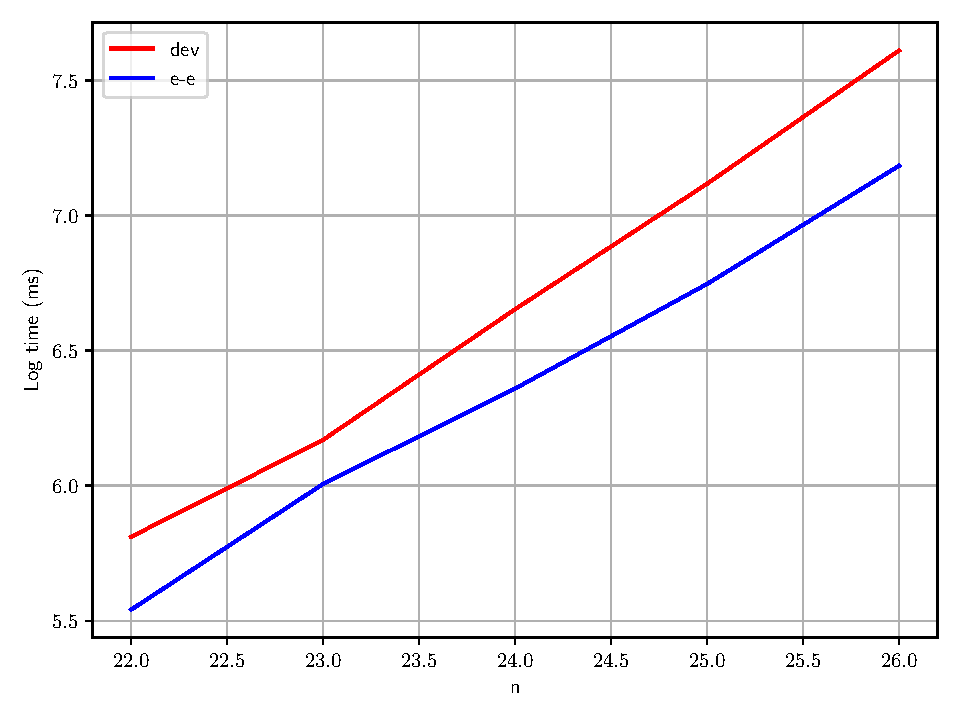
\includegraphics[width=0.7\textwidth]{img/perf_fib.pdf}
  \caption{Performance of evaluating $\text{fib}(n)$}
  \label{fig:perf-fib}
\end{figure}

\begin{figure}
  \centering
  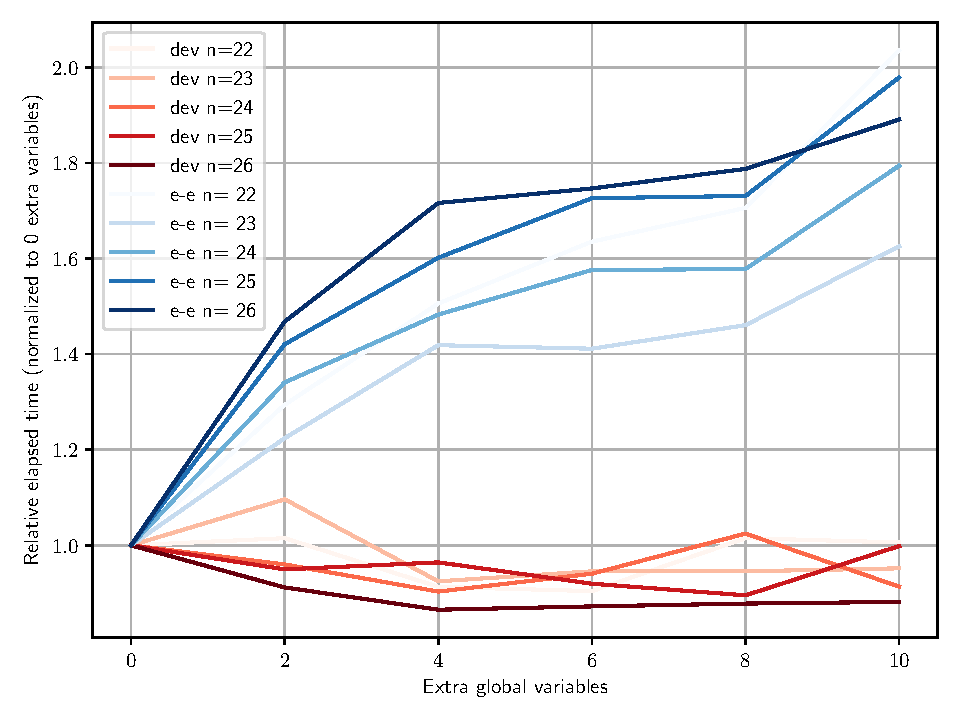
\includegraphics[width=0.7\textwidth]{img/perf_fib_more_vars.pdf}
  \caption{Performance of evaluating $\text{fib}(n)$ with extra global variables}
  \label{fig:perf-fib-more-vars}
\end{figure}

\begin{figure}
  \centering
  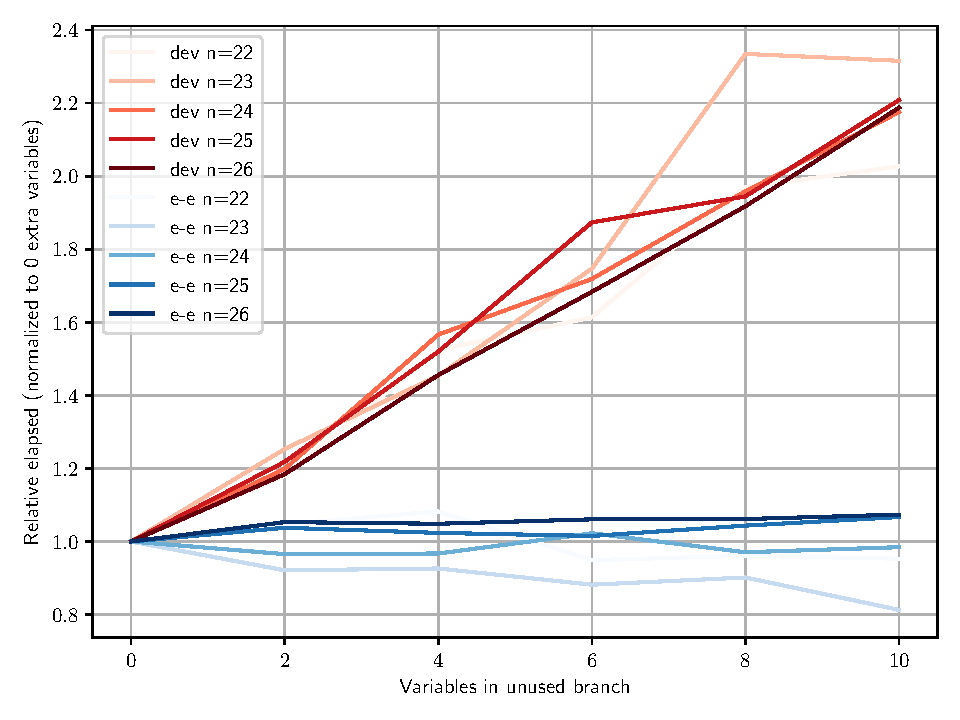
\includegraphics[width=0.7\textwidth]{img/perf_fib_more_branches.pdf}
  \caption{Performance of evaluating $\text{fib}(n)$ with an unused branch}
  \label{fig:perf-fib-more-branches}
\end{figure}


\section{Postprocessing performance}
\label{sec:evaluation-renumbering}

Consider the set of programs described by \Cref{fig:hole_renumbering_problem}.

\todo{describe this code blowup example}

\begin{singlespace}
  \begin{table}
    \centering
    \begin{tabular}{r|ccc|ccc}
      \hline
      & \multicolumn{3}{c|}{\texttt{dev} branch} & \multicolumn{3}{c}{\texttt{eval-environment} branch} \\
      & Evaluate & Postprocessing & Equality & Evaluate & Postprocessing & Equality \\
      \hline\hline
      1 & 0 & 0 & 0 & 0 & 1 & 0 \\
      2 & 0 & 0 & 0 & 0 & 1 & 0 \\
      3 & 1 & 2 & 0 & 0 & 1 & 0 \\
      4 & 1 & 1 & 1 & 1 & 0 & 0 \\
      5 & 1 & 1 & 2 & 0 & 3 & 0 \\
      6 & 5 & 1 & 3 & 1 & 0 & 0 \\
      7 & 4 & 5 & 6 & 2 & 2 & 0 \\
      8 & 3 & 3 & 14 & 0 & 0 & 0 \\
      9 & 6 & 18 & 33 & 1 & 0 & 1 \\
      10 & 14 & 29 & 61 & 0 & 0 & 0 \\
      11 & 13 & 41 & 91 & 3 & 2 & 0 \\
      12 & 25 & 145 & 203 & 2 & 0 & 1 \\
      13 & 65 & 578 & 383 & 2 & 0 & 0 \\
      14 & 147 & 2399 & 924 & 1 & 3 & 1 \\
      15 & 226 & 16597 & 1603 & 3 & 0 & 1 \\
      16 & & & & 1 & 0 & 1 \\
      17 & & & & 2 & 1 & 1 \\
      18 & & & & 0 & 3 & 1 \\
      19 & & & & 0 & 0 & 1 \\
      20 & & & & 3 & 4 & 0 \\
      21 & & & & 2 & 0 & 1 \\
      22 & & & & 0 & 2 & 1 \\
      23 & & & & 0 & 3 & 1 \\
      24 & & & & 0 & 6 & 1 \\
      25 & & & & 1 & 4 & 1 \\
      26 & & & & 1 & 2 & 1 \\
      \hline\hline
    \end{tabular}
    \caption{Performance of program illustrated in \Cref{fig:hole_renumbering_problem}}
    \label{tab:perf-hole-blowup}
  \end{table}
\end{singlespace}

\begin{figure}
  \centering
  \begin{subfigure}{0.7\textwidth}
    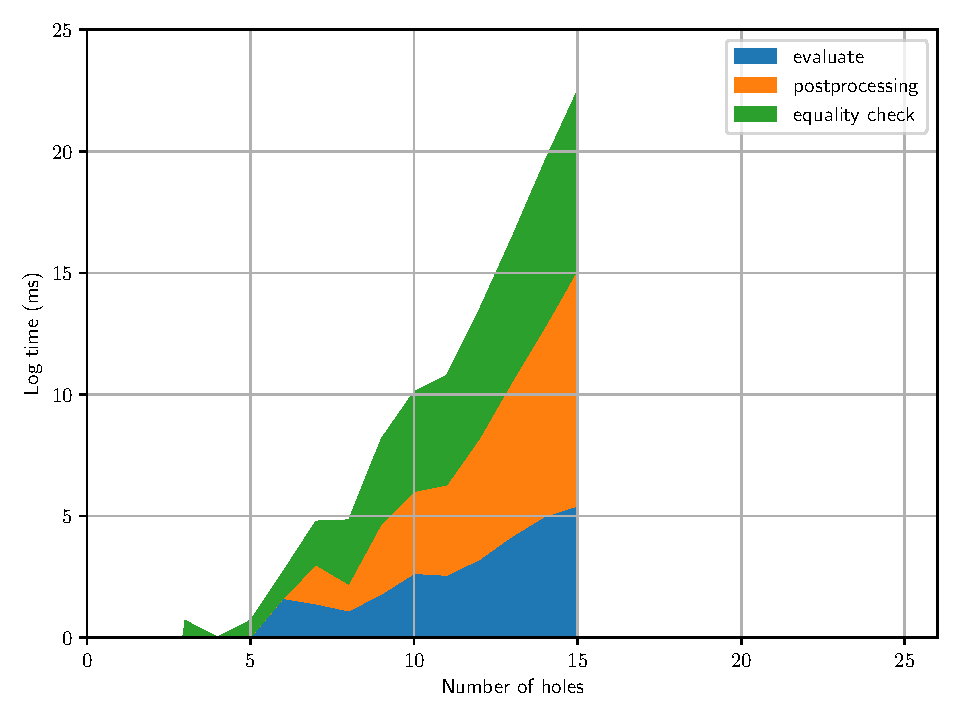
\includegraphics[width=\textwidth]{img/perf_renum_dev.pdf}
    \caption{\texttt{dev} branch}
    \label{fig:perf-renum-dev}
  \end{subfigure}
  \begin{subfigure}{0.7\textwidth}
    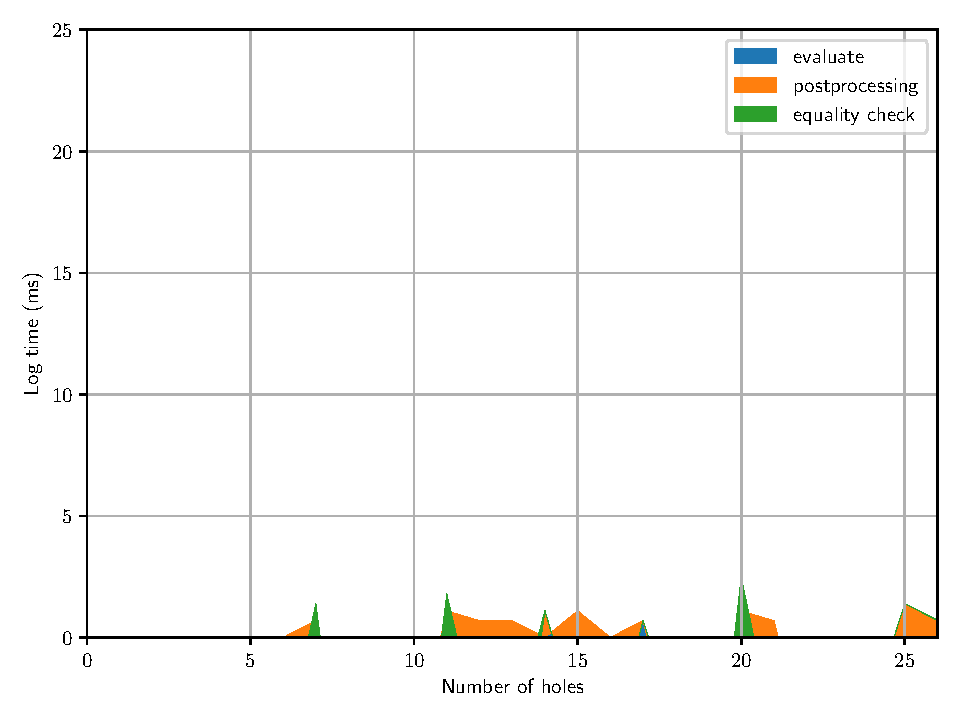
\includegraphics[width=\textwidth]{img/perf_renum_eev.pdf}
    \caption{\texttt{eval-environment} branch}
    \label{fig:perf-renum-eev}
  \end{subfigure}
  \caption{Performance of evaluating program in \Cref{fig:hole_renumbering_problem}}
  \label{fig:perf-renum}
\end{figure}

\section{FAR performance}
\label{sec:evaluation-far}

\begin{singlespace}
  \begin{table}
    \centering
    \begin{tabular}{p{10em}cccc}
      \hline
      Program & Steps & Steps & Step $\Delta$ & Cumulative \\
              & & (w/ FAR) & & Step $\Delta$ \\
      \hline\hline
      \inputhnfminted{far_fib_hist_1} & 7 & - & 0 & 0 \\ \hline
      \inputhnfminted{far_fib_hist_2} & 12 & 21 & 9 & 9 \\ \hline
      \inputhnfminted{far_fib_hist_3} & 17 & - & 0 & 9 \\ \hline
      \inputhnfminted{far_fib_hist_4} & 58 & 69 & 11 & 20 \\ \hline
      \inputhnfminted{far_fib_hist_5} & 4762964 & - & 0 & 20 \\ \hline
      \inputhnfminted{far_fib_hist_6} & 4762966 & 12 & -4762954 & -4762934 \\ \hline
      \inputhnfminted{far_fib_hist_7} & 4762966 & 21 & -4762954 & -9525879 \\ \hline
      \inputhnfminted{far_fib_hist_8} & 4792967 & 13 & -4792954 & -14288813 \\ \hline
      \hline
    \end{tabular}
    \caption{A program edit history with an expensive computation}
    \label{fig:far-program-history-fib}
  \end{table}
\end{singlespace}

\begin{singlespace}
  \begin{table}
    \centering
    \begin{tabular}{p{10em}cccc}
      \hline
      Program & Steps & Steps & Step $\Delta$ & Cumulative \\
              & & (w/ FAR) & & Step $\Delta$ \\
      \hline\hline
      \inputhnfminted{far_hist_1} & 1 & - & 0 & 0 \\ \hline
      \inputhnfminted{far_hist_2} & 2 & 3 & 1 & 1 \\ \hline
      \inputhnfminted{far_hist_3} & 3 & - & 0 & 1 \\ \hline
      \inputhnfminted{far_hist_4} & 4 & 5 & 1 & 2 \\ \hline
      \inputhnfminted{far_hist_5} & 5 & - & 0 & 2 \\ \hline
      \inputhnfminted{far_hist_6} & 6 & 9 & 3 & 5 \\ \hline
      \inputhnfminted{far_hist_7} & 8 & 8 & 0 & 5 \\ \hline
      \inputhnfminted{far_hist_8} & 9 & 14 & 5 & 10 \\ \hline
      \inputhnfminted{far_hist_9} & 10 & 11 & 1 & 11 \\ \hline
      \inputhnfminted{far_hist_10} & 11 & 6 & -5 & 6 \\ \hline
      \hline
    \end{tabular}
    \caption{A sample edit history for a simple program}
    \label{fig:far-program-history-simple}
  \end{table}
\end{singlespace}

\begin{figure}
  \centering
  \begin{subfigure}{0.7\textwidth}
    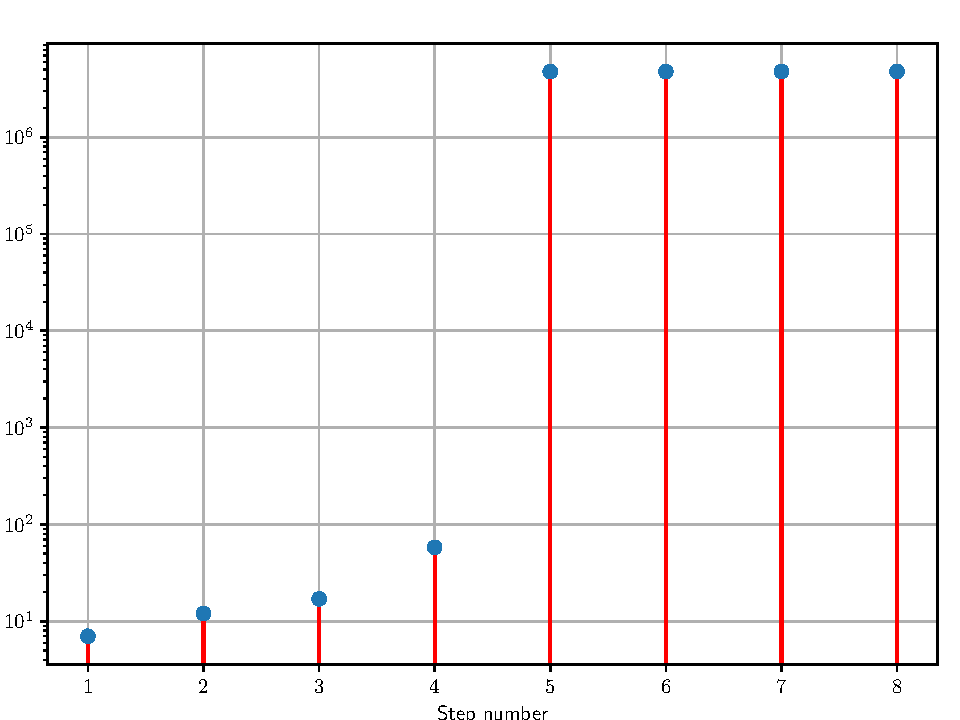
\includegraphics[width=\textwidth]{img/perf_no_far.pdf}
    \caption{Normal evaluation}
    \label{fig:perf-no-far}
  \end{subfigure}
  \begin{subfigure}{0.7\textwidth}
    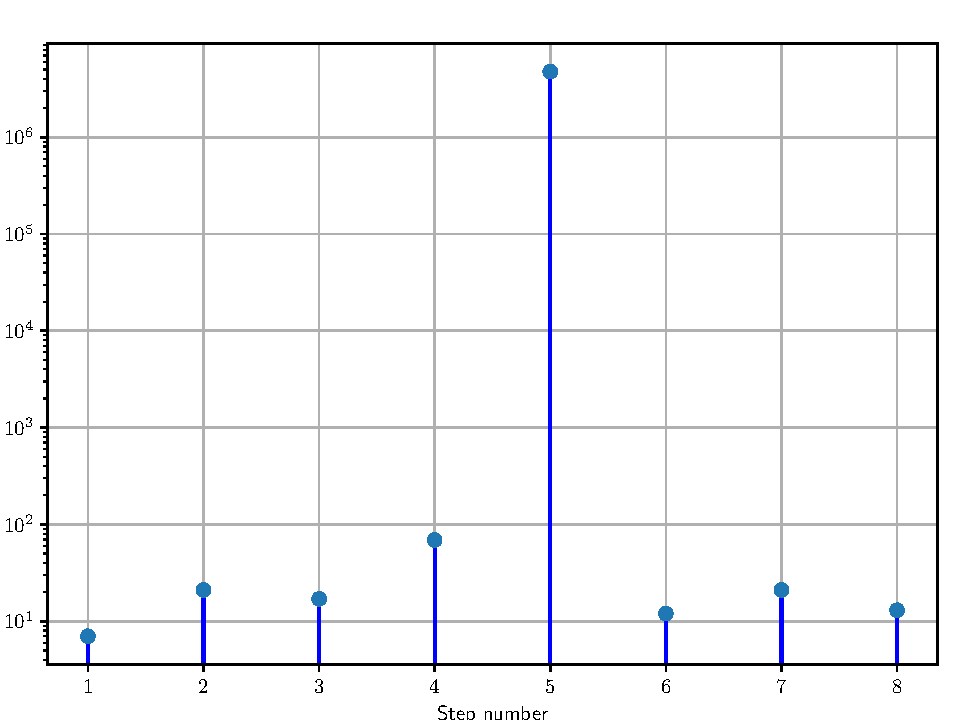
\includegraphics[width=\textwidth]{img/perf_far.pdf}
    \caption{With one-step FAR}
    \label{fig:perf-far-far}
  \end{subfigure}
  \caption{Number of evaluation steps per edit in \Cref{fig:far-program-history-fib}}
  \label{fig:perf-far}
\end{figure}

%%% Local Variables:
%%% mode: latex
%%% TeX-master: "main"
%%% End:
